% -*- latex -*-
%%%%%%%%%%%%%%%%%%%%%%%%%%%%%%%%%%%%%%%%%%%%%%%%%%%%%%%%%%%%%%%%
%%%%
%%%% This TeX file is part of the course
%%%% Introduction to Scientific Programming in C++/Fortran2003
%%%% copyright 2017-2020 Victor Eijkhout eijkhout@tacc.utexas.edu
%%%%
%%%% arrayj.tex : arrays in Julia
%%%%
%%%%%%%%%%%%%%%%%%%%%%%%%%%%%%%%%%%%%%%%%%%%%%%%%%%%%%%%%%%%%%%%

Reference: \url{https://docs.julialang.org/en/v1/manual/arrays/}

\Level 0 {Introduction}

Create array of length~3, with values undefined.
\begin{lstlisting}
Array{Int64}(undef,3)
\end{lstlisting}

Create array with 2 rows and 3 columns, with values undefined.
\begin{lstlisting}
Array{Integer}(undef, 2,3)
\end{lstlisting}

Zero-based indexing:
\begin{lstlisting}
mat = Array{Float64}(undef, 2,4)
typeof(mat)
show(mat)
mat[1,3] = 3.14
show(mat)
\end{lstlisting}

Bound checking:
\begin{lstlisting}
mat = Array{Float64}(undef, 2,4)
mat[2,4] = 3.14
mat[0,0] = 1.1
show(mat)
\end{lstlisting}

\Level 1 {Element access}

Julia uses the square bracket notation
\begin{lstlisting}
ar[5] = 6
\end{lstlisting}
with bounds that are 1-based.

(Fortran-style arbitrary lower bounds can be supported:
\url{https://docs.julialang.org/en/v1/devdocs/offset-arrays/})

\Level 1 {Arrays in linear algebra}
% https://docs.julialang.org/en/v1/stdlib/LinearAlgebra/

The keywords \lstinline{Vector} and \lstinline{Matrix}
are synonyms for
\begin{lstlisting}
Array{T,1}
Array{T,2}
\end{lstlisting}
respectively.

Additionally, there are
\begin{itemize}
\item  \lstinline{Symmetric}:	Symmetric matrix
\item  \lstinline{Hermitian}:	Hermitian matrix
\item  \lstinline{UpperTriangular}:	Upper triangular matrix
\item  \lstinline{UnitUpperTriangular}:	Upper triangular matrix with unit diagonal
\item  \lstinline{LowerTriangular}:	Lower triangular matrix
\item  \lstinline{UnitLowerTriangular}:	Lower triangular matrix with unit diagonal
\item  \lstinline{UpperHessenberg}:	Upper Hessenberg matrix
\item  \lstinline{Tridiagonal}:	Tridiagonal matrix
\item  \lstinline{SymTridiagonal}:	Symmetric tridiagonal matrix
\item  \lstinline{Bidiagonal}:	Upper/lower bidiagonal matrix
\item  \lstinline{Diagonal}:	Diagonal matrix
\item  \lstinline{UniformScaling}:	Uniform scaling operator
\end{itemize}

For some of these types, optimized addition and multiplication
routines are available.

\Level 1 {Type hierarchy}

There is an untyped base type \indexj{AbstractMatrix} from
which typed matrices are derived.
You can use the function \lstinline{eltype}
to find out what the type of an abstract matrix is:
\begin{lstlisting}
function look_at_matrix( A::AbstractMatrix )
  (size,type) = ( size(A,1),eltype(A) )
\end{lstlisting}

\Level 0 {Functions}

\Level 1 {Built-in functions}

\indexj{collect}: turn the elements of a collection or iterator
into an array. Example:
\begin{lstlisting}
integers = collect( 1:n )
\end{lstlisting}

\Level 1 {Scalar functions}

Scalar functions such as \indextermtt{abs} can be applied in a
\emph{pointwise}\index{function!pointwise application to array}
manner to an array by using a dot-notation.
Since this is ambiguous with taking a member of a structure,
the array needs to be enclosed in parentheses:

\snippetwithoutput{pointwisej}{arrayj}{pointwise}

\Level 1 {Vectors are dynamic}
\label{sec:vectorj-dynamic}

  An array
  can be grown or shrunk after its creation.
  For instance, you can use the \lstinline{push!} method to add elements at the end:

\begin{block}{Dynamic vector extension}
    \label{sl:vectorj-dynamic}
    Extend with \indextermtt{push!}:
    \snippetwithoutput{jarraypush}{arrayj}{push}
%% \begin{lstlisting}
%% c = [1]
%% for i in c
%%     push!(c, i)
%%     @show c
%%     sleep(1)
%% end
%% \end{lstlisting}
\end{block}

\Level 0 {Comprehensions}

It is possible to define an array by its elements.
\begin{lstlisting}
[i^2 for i in 1:10]
Complex[i^2 for i in 1:10]
[(i, sqrt(i)) for i in 1:10]
\end{lstlisting}

Two-dimensional:
\begin{lstlisting}
[(r,c) for r in 1:5, c in 1:2]
\end{lstlisting}

With a test to filter:
\begin{lstlisting}
[x for x in 1:100 if x % 7 == 0]
\end{lstlisting}

Enumerating:
\begin{lstlisting}
[i for i in enumerate(m)]
3x3 Array{Tuple{Int64,Int64},2}:
(1, 6)  (4, 5)  (7, 3)
(2, 4)  (5, 0)  (8, 7)
(3, 1)  (6, 7)  (9, 4)
\end{lstlisting}

Zip together multiple generators:
\begin{lstlisting}
for i in zip(0:10, 100:110, 200:210)
           println(i) 
end

(0,100,200)
(1,101,201)
(2,102,202)
(3,103,203)
(4,104,204)
(5,105,205)
(6,106,206)
(7,107,207)
(8,108,208)
(9,109,209)
(10,110,210)
\end{lstlisting}

You can iterators:
\begin{lstlisting}
ro = 0:2:100
[i for i in ro]
\end{lstlisting}

\Level 0 {Multi-dimensional cases}

Julia has support for multi-dimensional arrays.
Array types look like
\begin{lstlisting}
Array{Int64,2}  
\end{lstlisting}
for a two-dimensional array of \lstinline{Int64} objects.

\begin{block}{Array organization}
  Arrays are organized by columns. For instance using
  \indextermtt{reshape} to make a two-dimensional array
  from  one-dimensional one:
\begin{lstlisting}
a = reshape(1:100, (10, 10))
for n in a
    print(n, " ")
end
\end{lstlisting}
\end{block}

\begin{comment}
  \Level 1 {Matrix as vector of vectors}

  \begin{block}{Multi-dimensional vectors}
    \label{sl:multi-vector}
    Multi-dimensional is harder with vectors:
    \begin{lstlisting}
      vector<float> row(20);
      vector<vector<float>> rows(10,row);
      // alternative:
      vector<vector<float>> rows(10);
      for ( auto &row : rows )
      row = vector<float>(20);
    \end{lstlisting}
    Create a row vector, then store 10 copies of that:\\
    vector of vectors.
  \end{block}

  This is not the best implementation of a matrix, for instance because
  the elements are not contiguous. However, let's continue with it for a moment.

  \begin{block}{Matrix class}
    \label{sl:matrix-class}
    \verbatimsnippet{matrixclassdef}
  \end{block}

  \begin{exercise}
    \label{ex:matrixclass-rowcol1}
    Write \n{rows()} and \n{cols()} methods for this class that return
    the number of rows ad columns respectively.
  \end{exercise}

  \begin{exercise}
    \label{ex:matrix-methods}
    Add methods such as \n{transpose}, \n{scale} to your matrix class.

    Implement matrix-matrix multiplication.
  \end{exercise}

  \Level 1 {A better matrix class}

  You can make a `pretend' matrix by storing a long enough \n{vector} in
  an object:
  %
  \verbatimsnippet{matrixclass}

  \begin{slide}{Matrix class'}
    \label{sl:matrix-class-cont}
    Better idea:
    \begin{lstlisting}
      elements = vector<double>(rows*cols);
      ...
      void get(int i,int j) {
        return elements.at(i*cols+j);
      }
    \end{lstlisting}
    (Old-style solution: use cpp macro)
  \end{slide}

  \begin{exercise}
    \label{ex:matrixclass-rowcol2}
    Why are \lstinline{m,n} here stored explicitly, and not in the
    previous case?
  \end{exercise}

  The most important advantage of this is that it is compatible with
  the storage traditionally used in 
  many libraries and codes.

  The syntax for \n{set} and \n{get} can be improved.
  \begin{exercise}
    Write a method \n{element} of type \n{double&}, so that you can write
    \begin{lstlisting}
      A.element(2,3) = 7.24;
    \end{lstlisting}
  \end{exercise}

  \Level 0 {Advanced topics}

  \Level 1 {Iterators}
  \label{sec:iterator}

  You have seen how you can iterate over a vector
  \begin{itemize}
  \item by an indexed loop over the indices, and
  \item with a range-based loop over the indices.
  \end{itemize}
  There is a third way, which is actually the basic mechanism underlying
  the range-based looping.

  An \indexterm{iterator} is, in a metaphorical sense (see
  section~\ref{sec:iterator-class} for details) a pointer to a vector
  element. Mirroring the index-loop convention of
  \begin{lstlisting}
    for (int i=0; i<hi; i++)
    element = vec.at(i);
  \end{lstlisting}
  you can iterate:
  \begin{lstlisting}
    for (auto elt_ptr=vec.begin(); elt_ptr!=vec.end(); ++elt_ptr)
    element = *elt_ptr;
  \end{lstlisting}
  Some remarks:
  \begin{itemize}
  \item This is one of the very few places where you need the asterisk in C++
    for \indexterm{dereferencing}; section~\ref{sec:cderef}. (However,
    the thing you are dereferencing is an iterator, not a pointer.)
  \item As with a normal loop, the \n{end} iterator point just beyond the end
    of the vector.
  \item You can do \indextermbus{pointer}{arithmetic} on iterators, as
    you can see in the \verb-++elt_ptr- update part of the loop header.
  \end{itemize}
  Another illustration of pointer arithmetic on iterators is getting the
  last element of a vector:
  %
  \snippetwithoutput{vectorpush}{array}{vectorend}
  \snippetwithoutput[vectorend]{vectorpushiterator}{array}{vectorenditerator}

  \Level 1 {Old-style arrays}
  \label{sec:staticarray}

  Static arrays are really an abuse of the equivalence of arrays and
  addresses of the C programming language. This appears for instance in
  parameter passing mechanisms.

  For small arrays you can use a different syntax. 

  \snippetwithoutput{arrayinit}{array}{staticinit}

  This has the
  (minimal) advantage of not having the overhead of a class
  mechanism. On the other hand, it has a number of disadvantages:
  \begin{itemize}
  \item You can not query the size of an array by its name: you have to
    store that information separately in a variable.
  \item Passing such an array to a function is really passing the
    address of its first element, so it is always (sort of) by
    reference.
  \end{itemize}

  Range-based indexing works the same as with vectors:
  %
  \snippetwithoutput{rangemax}{array}{rangemax}

  \Level 2 {C-style arrays and subprograms}

  Arrays can be passed to a subprogram, but the bound is unknown there.
  %
  \verbatimsnippet{arraypass}
  %
  \begin{exercise}
    Rewrite the above exercises where the sorting tester or the maximum
    finder is in a subprogram.
  \end{exercise}

  Unlike with scalar arguments, array arguments can be altered by a
  subprogram: it is as if the array is always passed by reference. This is
  not strictly true: what happens is that the address of the first
  element of the array is passed. Thus we are really dealing with pass
  by value, but it is the array address that is passed rather than its value.

  \Level 2 {Multi-dimensional arrays}

  Multi-dimensional arrays can be declared and used with a simple extension of
  the prior syntax:
  \begin{lstlisting}
    float matrix[15][25];

    for (int i=0; i<15; i++)
    for (int j=0; j<25; j++)
    // something with matrix[i][j]
  \end{lstlisting}

  Passing a multi-dimensional array to a function, only the first
  dimension can be left unspecified:
  %
  \verbatimsnippet{arraypass2d}

  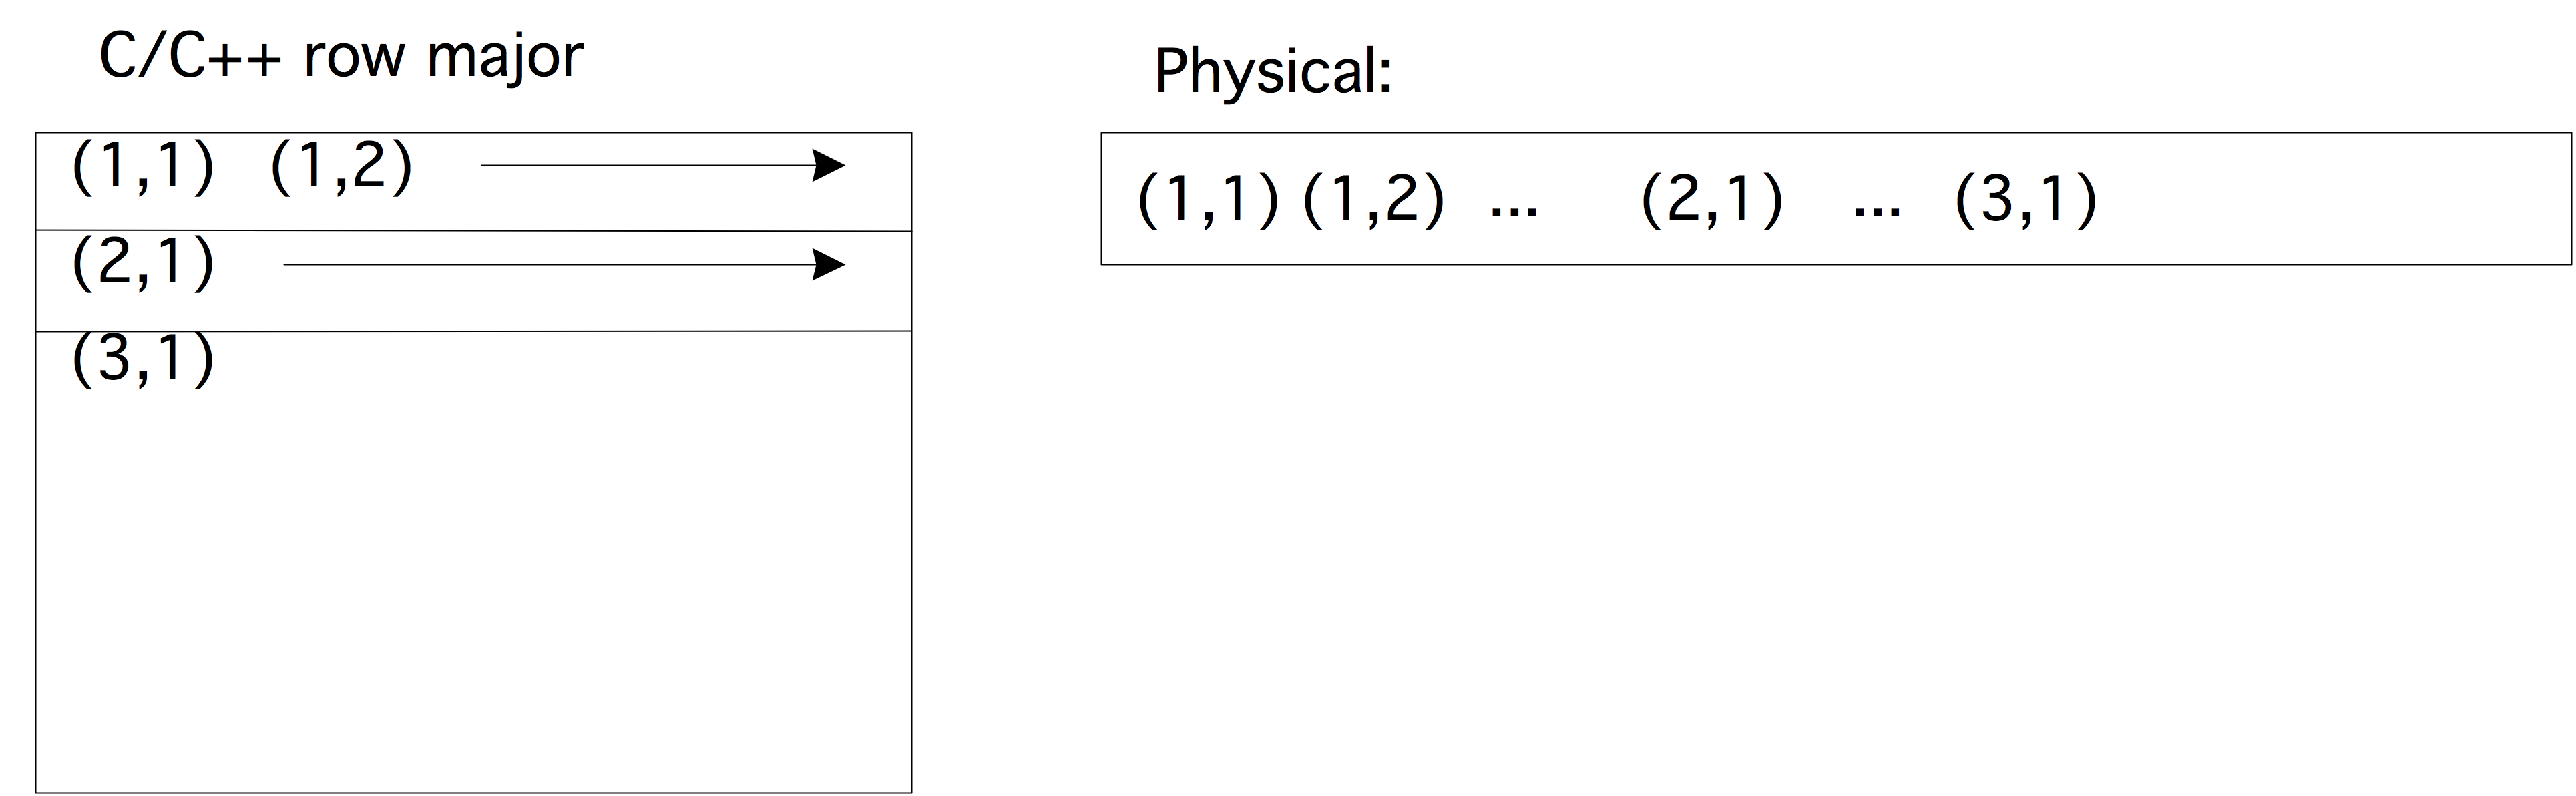
\includegraphics[scale=.1]{arrayc}

  \Level 2 {Memory layout}

  Puzzling aspects of arrays, such as which dimensions need to be
  specified and which not in a function call, can be understood by
  considering how arrays are stored in memory.
  The question then is how a two-dimensional (or higher dimensional)
  array is mapped to memory, which is linear.
  \begin{itemize}
  \item A one-dimensional array is stored in contiguous memory.
  \item A two-dimensional array is also stored contiguously, with first
    the first row, then the second, et cetera.
  \item Higher dimensional arrays continue this notion, with contiguous
    blocks of the highest so many dimensions.
  \end{itemize}

  As a result of this, indexing beyond the end of a row, brings you to the
  start of the next row:
  %
  \verbatimsnippet{arraywrap}

  We can now also understand how arrays are passed to functions:
  \begin{itemize}
  \item The only information passed to a function is the address of the
    first element of the array;
  \item In order to be able to find location of the second row (and
    third, et cetera), the subprogram needs to know the length of each
    row.
  \item In the higher dimensional case, the subprogram needs to know the
    size of all dimensions except for the first one.
  \end{itemize}

  \Level 1 {Stack and heap allocation}
  \label{sec:stack-heap}

  Entities stored in memory (variables, structures, objects) can exist
  in two locations: the \indextermdef{stack} and the
  \indextermdef{heap}.
  \begin{itemize}
  \item Every time a program enters a new
    \emph{scope}\index{scope!and stack}, entities declared there are
    placed on top of the stack, and they are removed by the end of the
    scope.
  \item The heap is for entities that transcend scope, for instance
    because they are pointed-to by a
    \emph{pointer}\index{pointer!and heap}.
    The space of such objects can be returned to the free store at any
    time, so the heap can suffer from
    \emph{fragmentation}\index{heap!fragmentation|textbf}.
  \end{itemize}

  The concepts of \indexterm{stack} and \indexterm{heap} do not appear
  in the \indextermbus{C++}{standard}. However, the following
  description generally applies:
  \begin{itemize}
  \item Objects that obey scope are allocated on the stack, so that
    their memory is automatically freed control leaves the scope.
  \item Dynamically created objects, such as the target of a pointer,
    live on the heap because their lifetime is not subject to scope.
  \end{itemize}
  The existence of the second category is a source of
  \indextermbus{memory}{leak}s in languages such as~C. This danger is
  greatly lessened in~C++.

  While in C the only way to create dynamic objects is by a call to
  \indextermtt{malloc}, in C++ a \indextermtt{vector} obeys scope, and
  therefore lives on the stack. If you wonder if this may lead to
  \indextermbus{stack}{overflow}, rest assured: only the descriptor, the
  part of the vector that remembers the size, is on the stack, while the
  actual data is on the heap. However, it is no longer subject to memory
  leaking, since the heap storage is deallocated when the vector object
  goes out of scope.

  If you want heap memory that transcends scope you can use the
  \indextermsub{smart}{pointer} mechanism, which also guarantees against
  memory leaks. See chapter~\ref{ch:pointer}.

  \Level 1 {The Array class}

  In cases where an array will never change size it would be convenient
  to have a variant of the \lstinline{vector} class that does not have
  the dynamic memory management facility.
  The \indextermttdef{array} class seems to fulfill this role at first sight.
  However, it
  is limited to arrays where the size is known at compile time.

  \Level 1 {Span}
  \label{sec:gsl-span}

  The old C~style arrays allowed for some operations that are harder to
  do with vectors. For instance, you could create a subset of an array with:
  \begin{lstlisting}
    double *x = (double*)malloc(N*sizeof(double));
    double *subx = x+1;
    subx[1] = 5.; // same as: x[2] = 5.;
  \end{lstlisting}
  In C++ you can write
  \begin{lstlisting}
    vector<double> x(N);
    vector<double> subx( x.begin()+1,x.end() );
  \end{lstlisting}
  but that allocates new storage.

  If you really want two vector-like objects to share data there is the
  \indextermttdef{span} class, which is in the \ac{STL} of
  \emph{C++20}\index{C++!C++20}. Until this standard is available you
  can use the \indexac{GSL}, for instance implemented in
  \url{https://github.com/Microsoft/GSL}.

  A span is little more than a pointer and a size, so it allows for the
  above use case. Also, it does not have the overhead of creating a
  whole new vector.

  \begin{block}{Span}
    \label{sl:spandef}
    \begin{lstlisting}
      vector<double> v;
      auto v_span = gsl::span<double>( v.data(),v.size() );
    \end{lstlisting}
    The \indextermtt{span} object has the same \lstinline{at}, \lstinline{data}, and
    \lstinline{size} methods, and you can iterate over it, but it has no
    dynamic methods.
  \end{block}

  \Level 0 {Exercises}

  \begin{exercise}
    Given a vector of integers, write two loops;
    \begin{enumerate}
    \item One that sums all even elements, and
    \item one that sums all elements with even indices.
    \end{enumerate}
    Use the right type of loop.
  \end{exercise}

  \begin{exercise}
    Program \indexterm{bubble sort}: go through the array comparing
    successive pairs of elements, and swapping them if the second is
    smaller than the first. After you have gone through the array, the
    largest element is in the last location. Go through the array again,
    swapping elements, which puts the second largest element in the
    one-before-last location. Et cetera.
  \end{exercise}

  \begin{block}{Pascal's triangle}
    \label{sl:pascal-def}
    \small
    \indexterm{Pascal's triangle} contains binomial coefficients:
              {\scriptsize
\begin{verbatim}
  Row    1:                     1
  Row    2:                   1   1
  Row    3:                 1   2   1
  Row    4:               1   3   3   1
  Row    5:             1   4   6   4   1
  Row    6:           1   5  10  10   5   1
  Row    7:         1   6  15  20  15   6   1
  Row    8:       1   7  21  35  35  21   7   1
  Row    9:     1   8  28  56  70  56  28   8   1
  Row   10:   1   9  36  84 126 126  84  36   9   1
\end{verbatim}
              }
              where \[ p_{rc} = \begin{pmatrix} r\\c \end{pmatrix} = \frac{r!}{c!(r-c)! }. \]
              The coefficients can be computed from the recurrence
              \[ p_{rc} = 
              \begin{cases}
                1&c\equiv 1\vee c\equiv r\\
                p_{r-1,c-1}+p_{r-1,c}
              \end{cases}
              \]
  \end{block}

  \begin{exercise}
    \label{ex:pascal-ex}
    \small
    \begin{itemize}
    \item 
      Write a class \n{pascal} so that \n{pascal(n)} is the object
      containing $n$~rows of the above coefficients. Write a method
      \n{get(i,j)} that returns the $(i,j)$ coefficient.
    \item
      Write a method \n{print} that prints the above display.
    \item
      Write a method \n{print(int m)} that prints a star if the
      coefficient modulo~$m$ is nonzero, and a space otherwise.
\begin{verbatim}
  *
  * *
  *   *
  * * * *
  *       *
  * *     * *
  *   *   *   *
  * * * * * * * *
  *               *
  * *             * *
\end{verbatim}
\item
  The object needs to have an array internally. The easiest solution
  is to make an array of size $n\times n$.
    \end{itemize}
  \end{exercise}

  \begin{exercise}
    \label{ex:pascal-ey}
    Extend the Pascal exercise:\\
    Optimize your code to use
    precisely enough space for the coefficients.
  \end{exercise}

  \begin{exercise}
    A knight on the chess board moves by going two steps horizontally or
    vertically, and one step either way in the orthogonal
    direction. Given a starting position, find a sequence of moves that
    brings a knight back to its starting position. Are there starting
    positions for which such a cycle doesn't exist?
  \end{exercise}

  \begin{exercise}
    Put eight queens on a chessboard so that none threatens any other.
  \end{exercise}

  \begin{exercise}
    From the `Keeping it REAL' book, exercise 3.6 about Markov chains.
  \end{exercise}
\end{comment}
